\documentclass[version=last,fontsize=13pt]{scrartcl}

\usepackage{pdfpages}
\usepackage{graphicx}

\usepackage{indentfirst}

\usepackage{titlesec}
\usepackage{caption}

\titlespacing*{\section}{0pt}{3ex}{3ex}
\titlespacing*{\subsection}{0pt}{1.5ex}{1.5ex}
\titlespacing*{\subsubsection}{0pt}{1.5ex}{1.5ex}

\usepackage[margin = 0.8in]{geometry}

%my own paragraph for which the text that follows starts on a new line
\newcommand{\myparagraph}[1]{\paragraph{#1}\mbox{}\\}

% dont number sections
% \setcounter{secnumdepth}{0}

\usepackage{wrapfig}
\usepackage{float}

\usepackage{caption}
\usepackage{subcaption}

\usepackage{tabularx}
\usepackage{appendix}

\usepackage{caption}
\usepackage{subcaption}
\usepackage{blindtext}

%settings for providing quotes
\def\signed #1{{\leavevmode\unskip\nobreak\hfil\penalty50\hskip2em
  \hbox{}\nobreak\hfil(#1)%
  \parfillskip=0pt \finalhyphendemerits=0 \endgraf}}

\newsavebox\mybox
\newenvironment{aquote}[1]
  {\savebox\mybox{#1}\begin{quote}}
  {\signed{\usebox\mybox}\end{quote}}

\usepackage{hyperref}


\begin{document}

\begin{titlepage}
	\begin{center}	
		
\includegraphics[width = 5cm,height = 1.5cm]{./imgs/uws_logo.png}\\[5cm]

	{ \huge \bfseries %
		Development and evaluation of a Mobile Web booking application for youth work\\ \Large 
}
	\vspace{2cm}
	
	\vspace{2cm}			
			

			
		\begin{flushright}
				\large Student:\\
				Marius-Lucian Olariu\\[1cm]
		\end{flushright}
		
	
		\begin{flushleft}
			 \large
				Supervisor: \\
				Dr. Daune West \\[1cm]
		\end{flushleft}
		
	\vspace{2cm}	
	
		
		\vfill

			{\large {Paisley \\ Word count: ? \\ 2019}}
		\end{center}
\end{titlepage}

\renewcommand{\labelenumi}{\roman{enumi}}

\newpage

\tableofcontents

\newpage

\listoffigures

\newpage

\section{Abstract}(5 p - 300w )\\
% Summary of the problem, core problems and how these will be
% addressed. Please include up to 5 key words or phrases at the bottom of the abstract.
% (maximum 300 words – please give word count in document) 
A pilot study on the development of a Mobile Web system (mobile app and webpage) for YMCA Paisley.

\section{Aims}(5 p - 125w )\\
% General statements on intent and direction of the research
The main aim of this work is to develop a prototype webpage and a mobile application for the YMCA Paisley. This software system would provide valuable insights for the organization regarding their activity and how it can be improved using the mobile and web technology. Moreover, once the study is finished the organisation can decide if it's worth to commission the development of such a system by a company or not. 

\section{Objectives}(10 p - 250w)\\
% A list of clear, measurable statements of intended outcomes. i.e. What you are going to do in order to answer the question in the title and how you are going to do this (in relative detail) 

\section{Justification}(5 p - 125 w)\\
 % Rationale for the research showing gaps in current knowledge
% and how the results of the research might be used.
% (Aims, Objectives, Justification – about 1 page) (5 marks)

\pagebreak

\section{Review of the literature } (20p - 1700w - 2000w)\\
	% Review of Literature: History of problem with key sources with critical appraisal of contributions.
% (guidance - no more than 2000 words – please give word count in document)
% (20 marks)

%FIXME should I remove the subsections?
\subsection{Usability for Mobile-Web}

\indent
	The world of phones and computing changed in 2007 when the first iPhone was released due to the fact that this phone allows users to access Internet, has a touchscreen interface and is essentially a small computer that fits in a pocket. The term \textit{smartphone} is used to describe such a device. At the time of writing of this work (2019) there are about 2.71 billion smartphone users around the world and the number is expected to increase in the future (Number of smartphone users worldwide 2014-2020, n.d.). Such a large pool of users drives big companies to invest in their mobile applications and their websites in order to provide better customer experience (Vagrani, Kumar and Ilavarasan, 2017).\\ 
	All major airlines companies nowadays offer booking facilities both through their website and mobile app. In this work the term mobile-web app is going to describe a webpage accompanied by a mobile app. While the purpose of this work is not related to any e-commerce industry, it is still worth to analyze how these booking systems are designed in  order to develop a better mobile-web prototype app. One of the crucial factors for using a mobile-web app from the perspective of the users is \textit{usability} and \textit{user experience}. However, there are different opinions in literature to what these terms mean. To eliminate any confusion that might arise their definitions from ISO 9241-210:2010 (2010) are provided below.

\begin{aquote}{ISO 9241-210:2010, 2010, non-paginated}
	\textit{User Experience - person's perceptions and responses resulting from the use and/or anticipated use of a product, system or service.}	
\end{aquote}

\begin{aquote}{ISO 9241-210:2010, 2010, non-paginated}
	\textit{Usability -
extent to which a system, product or service can be used by specified users to achieve specified goals with effectiveness, efficiency and satisfaction in a specified context of use}	
\end{aquote}

The user experience and usability have common characteristics, however, the former is harder to evaluate (McNamara and Kirakowski, 2005) thus we will discuss focus  on usability.
The design of a webpage is not affected by many variables as it's the case for a mobile app. When designing a mobile app one has to take into account that the user might be on the move, a variable screen size, attention interruptions or poor network connection (Oulasvirta et al, 2005). Following their study on usability for a mobile flight booking app Gündüz and Pathan (2012) have identified  usability challenges that are going to be briefly detailed. Icons help in saving screen space and aid in completion of tasks, however, \textit{the wrong choice of icons} leads to confusion, it is suggested to use the same icons on web and mobile app to have consistency. Next, the mobile interface needs  to have \textit{a smaller number of steps} compared to the web app to achieve a task (e.g. search for flights) due to the fact that network interruptions might occur. Subsequently, the user inputs in a mobile app should be located towards the bottom of the screen to \textit{favor single hand use of the device}. Lastly,  there should not be presented a lot of information at once (cognitive overload) and the most important bits should be highlighted (e.g. departure and return date for a flight).

	\subsection{Cross-platform development approach}
	%mby add a bit about the web
	The mobile app needs to be developed for both major mobile \textbf{o}perating \textbf{s}ystems (OS), namely, Android and iOS. This implies  to write the code for the application twice, once in Java  for Android and once in Swift for iOS, this approach is known as native app development. While this is the ideal way to obtain app performance it is not feasible given the total time allowed for a MSc project. Therefore, to save time one can use a \textbf{c}ross-\textbf{p}latform \textbf{t}ool (CPT) where the codebase is written just once and the CPT generates an applcation for multiple mobile OSs. However, there are many CPTs available and it is hard to choose one that best fits a project without prior research. To get an ideea of how many options are available, for instance, in an industry report by SlashData (2012) there were discussed more than 100 CPTs. The same report (SlashData, 2012) higlights that developers' satisfaction regarding CPTs has been low, however, the author believes that some CPTs are now mature and better suited for development. \\
	\indent
	There are 5 types of CPTs: i) app factories, ii) source code translators, iii) JavaScript frameworks, iv) runtimes and v) Web-to-Native. The app factories target non-developers and help them to create a basic app by using drag-and-drop visual elements (the process is similar to solving a puzzle). JavaScript frameworks allows web developers to develop mobile apps using client-side technologies (HTML, CSS and JavaScript) the resulting mobile app is basically a webpage for mobile that can be accessed through a mobile browser. Web-to-Native are similiar to JavaScript frameworks in terms of development technologies just that this CPT packs the mobile website into a standalone mobile app that can be installed on the devices. 
	%Runtime CPTs have their own language for writing the app code which is directly complied to executable code for a mobile OS. 
	Runtime CPTs allow developers to write the non-native app using a language like Java and provide a special runtime for executing it for each mobile OS; basically,  the native app is comprised of the non-native part and the runtime that executes it.  
	Source code translators CPTs allow one to write the app code in a specific language which later is translated to the equivalent code for a specific mobile OS (e.g. Java/Swift) which in turn is compiled to executable code.\\
	\indent
	A complex analysis of 10  CPTs was done by Willocx, Vossaert and Naessens (2016) resulting in a series of guidelines for picking a CPT. Apps developed with JavaScript frameworks stress more the CPU and consume more memory than native apps, however, their performance is comparable to their native counterparts. The size of the app installer and the memory consumption is increased when using runtime CPTs compared to a native app. The best choice from a technical perspective it seems \textit{source code translators} that provide performances comparable with the native approach. Apart from these technical considerations, there are some non-technical considerations that can help in decision process: existing infrastructure (Webpages can be directly converted to mobile using JavaScript CPTs), skills of developer (one can pick a CPT that uses technologies he knows), flexibility (some CPTs offer better support to access OS specific features) and type of application (some CPTs are better for developing game apps). Given the above guidelines the author is going to use Flutter (n.d.), a CPT developed by Google, which is a source code translator according to the above classification because the performance of the app will be close to the native counterpart.

	%it is reasonable to look to use a cross platform development tool. To analyse which options are the best I read a paper
\section{Methodology}(25 p - 1000w)\\
	 % Explanation and justification of approach and methodology proposed. This section should explain the nature of the data you expect to collect; who will be involved and how you will collect it? Clear signposting of selection process of organisations/groups/individuals involved in the study should be explained. Identification and brief discussion of any analytical tools to be used; Identification of any ethical issues.
% (guidance – no more than 1000 words – please give word count in document) 

%likeart-type scale

\pagebreak
\section{Work plan}(10p - )\\
%do I need to write smth here or the gantt chart is enough?
\blindtext

	\begin{figure}[H]

		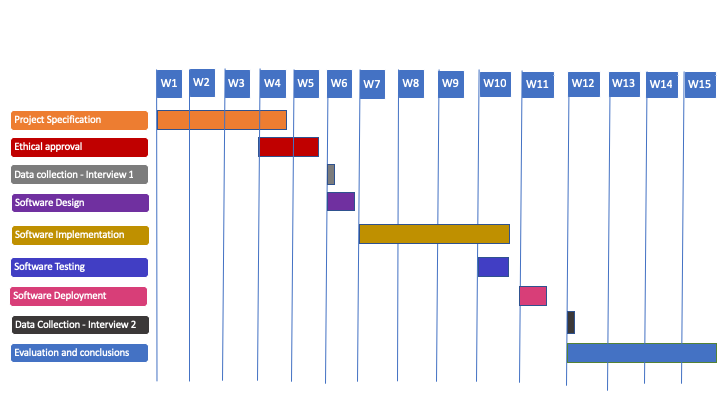
\includegraphics[scale = 0.5]{./imgs/ganttChart}
		\caption{All the activities that need to be undertaken to finish the project}
		\label{gC}

	\end{figure}

\pagebreak
\section*{References}

\underline{Flutter} (n.d.) [Online] Available: https://flutter.dev [Accessed 5 Apr 2019]\\

Gündüz, F. and Pathan, A.S.K., (2012) Usability improvements for touch-screen mobile flight booking application: A case study.  \underline{International Conference on Advanced } \underline{Computer Science Applications and Technologies}  pp. 49-54. Kuala Lumpur: IEEE.\\

\underline{ISO 9241-210:2010} (2010) [Online] Available: https://bit.ly/1j1dMhv [Accessed 3 Apr 2019].\\

McNamara, N. and Kirakowski, J., (2005)  Defining usability: quality of use or quality of experience? In \underline{IPCC 2005. Proceedings. International Professional Communication} \underline{Conference} pp. 200-204. Limerick: IEEE.\\

\underline{Number of smartphone users worldwide 2014-2020} (n.d.) [Online]  Available:\\ https://bit.ly/2dk8wHh [Accessed 3 Apr 2019].\\

Oulasvirta, A., Tamminen, S., Roto, V. and Kuorelahti, J., (2005) Interaction in 4-second bursts: the fragmented nature of attentional resources in mobile HCI. \\
\underline{In Proceedings of the SIGCHI conference on Human factors in computing systems} pp. 919-928. New York: ACM. \\

SlashData (2012) \underline{Vision mobile cross-platform developer tools 2012}  [Online] Available: https://bit.ly/2GhaYMC [Accessed 5 Apr 2019].\\

Vagrani, A., Kumar, N. and Ilavarasan, P.V., (2017) Decline in Mobile Application Life Cycle. \underline{Procedia computer science}. vol. 122, pp. 957-964. [Online] Article in Press. Available: https://doi.org/10.1016/j.procs.2017.11.460 [Accessed 3 Apr 2019].\\

Willocx, M., Vossaert, J. and Naessens, V. (2016) Comparing performance parameters of mobile app development strategies.  \underline{2016 IEEE/ACM International Conference on} \underline{Mobile Software Engineering and Systems (MOBILESoft)} pp. 38-47.  Austin: IEEE.\\

\end{document}

